\documentclass[../main.tex]{subfiles}


\begin{document}

\section{Approach}

Our detailed approach is constructed as follows:

\subsection{Method Declaration}

STCD is based on methods, it counts tokens in each method. So the very first thing to do is method declaration. Here we used ASTParser Tool to catch each method and get the information, which means, the \textit{startLineNumber, endLineNumber, methodName, methodParameters, methodType, methodBody}. This costs extra time than needed and can be improved in future work.

\subsection{Tokenization}

Since we have divided the whole file into methods, next is to tokenize the method body and get the frequency of each token. Comments and white-spaces removal process are included.

\subsection{Categorization}

Now for each method, we have a list of tokens, these tokens fall into 9 categories: \textit{methodParameter, methodType, tokenListNumber, tokenListType, tokenListKeyword, tokenListMarker, tokenListOperator, tokenListOther1, tokenListOther2}. The purpose of doing so is that these categories have different importance. For example, two pieces of codes both have 2 type names: ``int'', that provides little useful information, however, if two pieces of codes both have 2 variable names: ``drawVerticalLine'', that means this pair of codes are more likely the same. Later on these categories will be given different weights, depending on their importance.

A list of categorized tokens is shown in Table \ref{tab:Table_1}.

\begin{table}[t]
\footnotesize
\setlength{\abovecaptionskip}{0pt}
\setlength{\belowcaptionskip}{0pt}
\caption{A List of Token Frequency}\label{tab:Table_1}
\begin{tabular}{|c|c|c||c|c|c|}
\hline
\textbf{Token} & \textbf{Category} & \textbf{Freq} & \textbf{Token} & \textbf{Category} & \textbf{Freq}\\
\hline
int & Type &1 		&  ) & Marker & 6\\
\hline
for & Keyword & 1 	& \} & Marker & 2\\
\hline
i & Other1 & 8		& \{ & Marker & 1\\
\hline
System & Other1 & 3	& + & Operator & 6\\
\hline
out & Other1 & 3	& = & Operator & 1\\
\hline
println & Other1 & 3	& - & Operator & 1\\
\hline
toBinary & Other1 & 1	& < & Operator & 1\\
\hline
Integer & Other1 & 1	& : & Other2 & 2\\
\hline
toBinaryString & Other1 & 1	& 5.0 & Num & 1\\
\hline
( & Marker & 6		& 33.0 & Num & 1\\
\hline
\end{tabular} \\
\end{table}

\subsection{Pre-processing of Variable Names}

Among all the categories, \textit{ tokenListOther1}, i.e. variable name is special. Its similarity is calculated with bigram algorithm\cite{bigram}. If ``drawVerticalLine'' and ``VerticalDrawLine'' appear in two code fragments respectively, we do not want to take them as different. So two variable names will be compared by bigram algorithm, if they are similar, they will be considered as the same and their frequencies will be compared later.

\subsection{Similarity Calculation for Each Category}

After the pre-processing of variable names, similarity algorithms are applied to these categories. For ``tokenList'' categories, tokens with their frequencies can be taken as a list, so the similarity for two lists can be calculated. We have 9 similarity values for these categories.

\subsection{Final Similarity Calculation and Result}

Finally, the 9 similarity values are given different weights and the final similarity will be calculated. A threshold is introduced, if the final similarity is higher than the threshold, the result will be printed out in the following format: clone group number, similarity value: method name 1, start line number, end line number; method name 2, start line number, end line number.

%\begin{figurehere}
%\centering 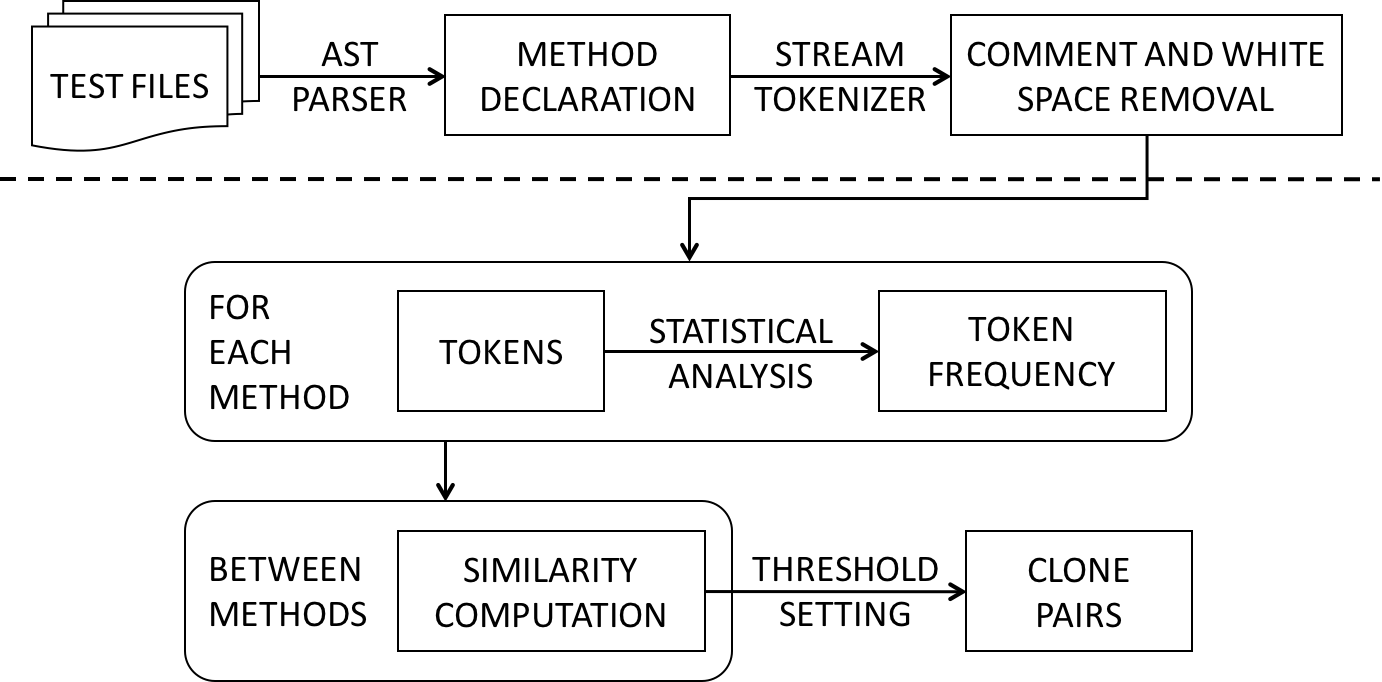
\includegraphics[width = 0.45 \textwidth]{Graph_1} 
%\caption{Overall Project Framework} \label{fig:Graph_1}
%\end{figurehere}

\subsection{Multilayer Perceptron}

During the final step, different weights are given to different categories, however, picking 9 weights arbitrarily may not be reasonable. So we used machine learning method to improve the results. Provided training files with ``ground truth'', a multilayer perceptron(MLP) is introduced to achieve this goal. 

MLP\cite{mlp} is an artificial neural network model that maps sets of input data onto a set of appropriate outputs. A single MLP contains three layers of nodes, and the nodes in one layer are fully connected with those in the next one. To train the network, this model utilizes back-propagation which is a supervised learning technique.
After actual testing, it turns out MLP does provide a better result.

A diagram describing the whole process is shown in Fig. \ref{fig:Graph_2}.\\

\begin{figurehere}
\centering 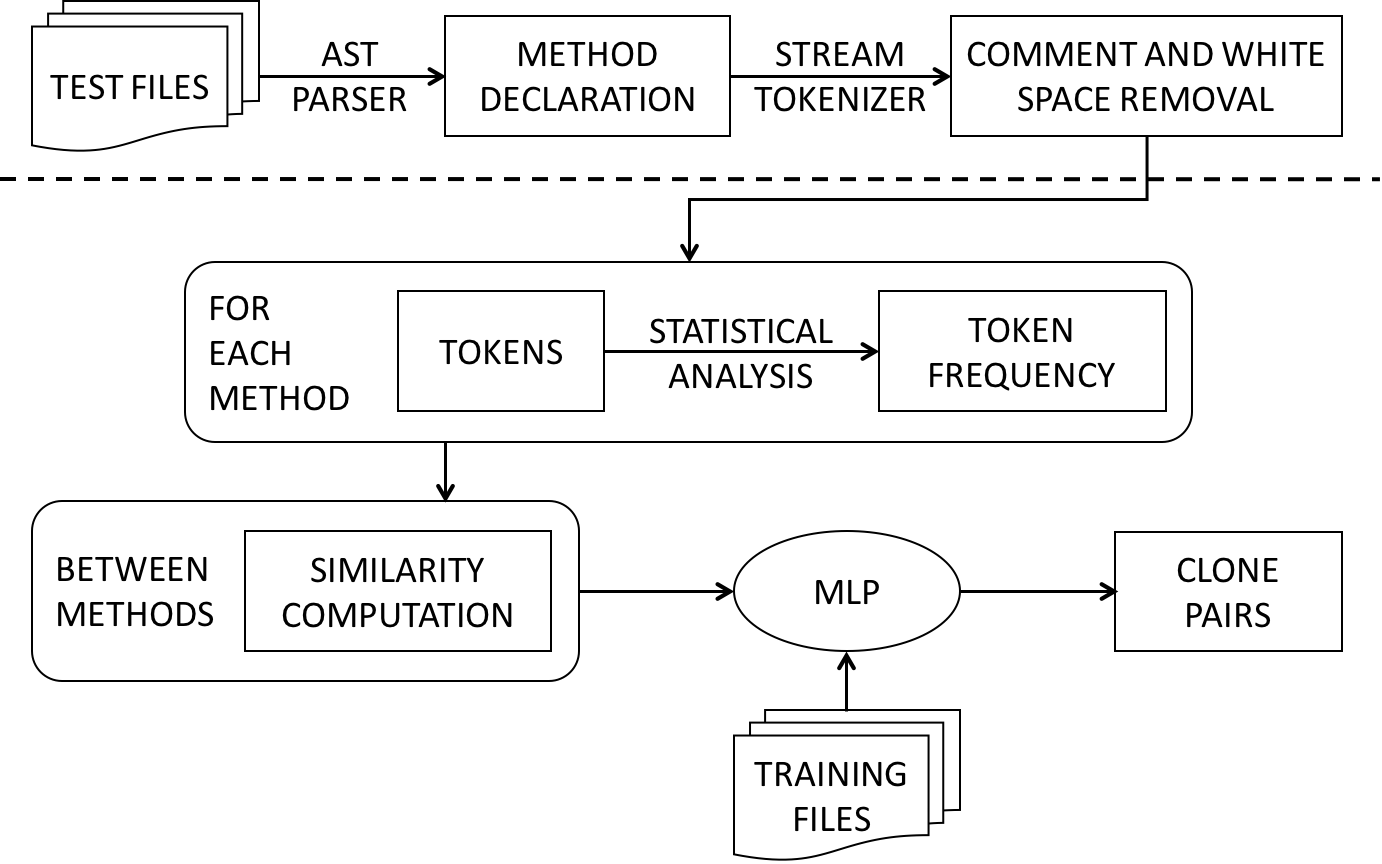
\includegraphics[width = 0.4 \textwidth]{Graph_2} 
\caption{Overall Project Framework} \label{fig:Graph_2}
\end{figurehere}

\end{document}